%======================================================================
%----------------------------------------------------------------------
%               XX                              X
%                                               X
%               XX    XXX   XXX   XXX      XXX  X  XXXX
%                X   X   X X   X X   X    X   X X X
%                X   XXXXX XXXXX XXXXX    X     X  XXX
%                X   X     X     X     XX X   X X     X
%               XXX   XXX   XXX   XXX  XX  XXX  X XXXX
%----------------------------------------------------------------------
%  	         A SKELETON FILE FOR IEEE PAPER GENERATION
%----------------------------------------------------------------------
%======================================================================

% first, uncomment the desired options:
\documentclass[%
        %draft,
        %submission,
        %compressed,
        final,
        %
        %technote,
        %internal,
        %submitted,
        %inpress,
        %reprint,
        %
        %titlepage,
        notitlepage,
        %anonymous,
        narroweqnarray,
        inline,
        %twoside,
        ]{ieee}
%
% some standard modes are:
%
% \documentclass[draft,narroweqnarray,inline]{ieee}
% \documentclass[submission,anonymous,narroweqnarray,inline]{ieee}
% \documentclass[final,narroweqnarray,inline]{ieee}

% Use the `endfloat' package to move figures and tables to the end
% of the paper. Useful for `submission' mode.
%\usepackage {endfloat}

% Use the `times' package to use Helvetica and Times-Roman fonts
% instead of the standard Computer Modern fonts. Useful for the 
% IEEE Computer Society transactions.
% (Note: If you have the commercial package `mathtime,' it is much
% better, but the `times' package works too).
%\usepackage {times}

% In order to use the figure-defining commands in ieeefig.sty...

\usepackage[spanish]{babel}
\usepackage[utf8]{inputenc}
\usepackage{ieeefig}

\usepackage{amssymb,amsmath}
\numberwithin{equation}{section}
\numberwithin{figure}{section}
\numberwithin{table}{section}
%\usepackage[dvipdfm,colorlinks=true,linkcolor=black,urlcolor=blue]{hyperref}
%\usepackage[hang,bf]{caption}

\newcommand{\imgdir}{tp-img}
\graphicspath{{\imgdir/}}

\begin{document}

%----------------------------------------------------------------------
% Title Information, Abstract and Keywords
%----------------------------------------------------------------------
\title[Implementación de un detector QRS]{%
       Detector de QRS basado en el algoritmo de Pan y Tompkins}

% format author this way for journal articles.
\author[SERGIO HINOJOSA]{%
      Sergio Hinojosa%\member{Estudiante}
      \authorinfo{%
      S. Hinojosa is with the Facultad de Ingeniería,
      Universidad de Buenos Aires, Buenos Aires, Argentina,
      email: \mbox{shinojosa@fi.uba.ar}}
  }

% specifiy the journal name
\journal{Señales e Imágenes en Biomédicina, 1er cuatrimestre 2011}

% Or, when the paper is a preprint, try this...
%\journal{IEEE Transactions on Something, 1997, TN\#9999.}

% Or, specify the conference place and date.
\confplacedate{Buenos Aires, Argentina, Enero 29, 2012}

% make the title
\maketitle               

% do the abstract
\begin{abstract}
En el siguiente trabajo se presenta una implementación y evaluación del algoritmo de detección de complejos QRS en señales de electrocardiografía basado en el algoritmo de Jiapu Pan y Willis J. Tompkins. Dicha implementación fué realizada en Python y se evaluó su performance utilizando la base de datos de arritmias del Instituto Tecnológico de Massachusetts (MIT) y el Hospital Beth-Israel (de aquí en adelante MIT-BIH) publicadas en el banco de señales Physionet.
\end{abstract}

% do the keywords
\begin{keywords}
Detector QRS, Pan y Tompkins, Python.
\end{keywords}

% start the main text ...
%----------------------------------------------------------------------
% SECTION I: Introduction
%----------------------------------------------------------------------
\section{Introducción}

\PARstart El complejo QRS contiene importante información clínica, por ejemplo su frecuencia de aparición puede proporcionar información sobre la actividad del sistema nervioso autonómo. Si bien su relación señal ruido es mucho mayor que otras señales bioléctricas, su detección es afectada por artefactos debido a ruido muscular, movimiento de electrodos, interferencia de línea, corrimiento de la línea de base, y ondas T de alta frecuencia.

	Dada la gran cantidad de estudios que requieren el delineado de la señal, y por lo tanto la localización de los complejos QRS, y las dificultades mencionadas asociadas a su detección, resulta esencial disponer de un algoritmo de detección robusto y confiable capaz de detectar tales marcas en condiciones de mucho ruido o de señal muy alterada por causas fisiológicas.

	En este sentido, el algoritmo de detección de complejos QRS desarrollado por Jiapu Pan y Willis J. Tompkins ha alcanzado un gran reconocimiento en la comunidad científica por su alto valor predictivo.
	
\section{Método}

La figura \ref{fig:pasos} muestra los pasos del proceso de análisis y en la figura \ref{fig:evolucion} 
se ve la evolucion de un latido tipo que aparece en la figura \ref{fig:evolucion}(a). 
Primero, se filtra la señal con un
filtro pasabanda que permite obtener solo la banda donde se espera encontrar los complejos
QRS y elimina otras señales que interfieren en la detección. Esto se realiza con un filtro pasa
bajos que elimina todo el ruido de alta frecuencia (lo cual incluye por ejemplo, el
ruido de 50Hz de la red de alimentación) y con un filtro pasa altos que como se
ve, elimina las componentes de continua y las ondas P y T (figura \ref{fig:evolucion}(b)). Luego, se deriva la señal filtrada
para detectar las pendientes pronunciadas características de los complejos QRS.
Hasta aquí el procesamiento es lineal, pero a continuación se realiza una medida de la
energía instantánea de la derivada de la señal elevando al cuadrado muestra a muestra
y promediando mediante una integral móvil $(E[x(t)] =< x^2 > |^t_{t-\tau})$. Esta medida de la
energía permite: primero, que cuando la señal es elevada al cuadrado todas las muestras sean
positivas y se acentúe la diferencia entre las distintas pendientes detectadas en la etapa de
diferenciación (figura \ref{fig:evolucion}(c)); segundo, cuando se promedia se eliminan las oscilaciones de poca
duración que no pueden corresponder a un complejo QRS y se obtiene un pulso uniforme
en la sección de señal correspondiente a un complejo QRS (figura \ref{fig:evolucion}(d)).

\begin{figure}
	\centering
	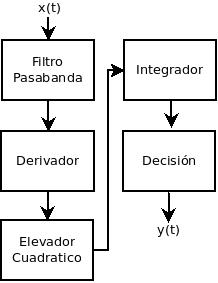
\includegraphics[width=4 cm]{diagrama1}
	\caption{Bloques del procesamiento}
	\label{fig:pasos}
\end{figure}

\begin{figure}
	\centering
	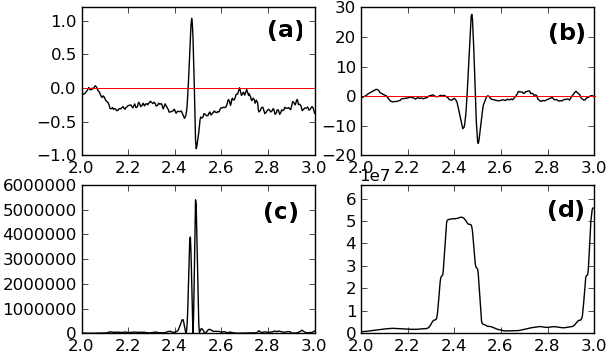
\includegraphics[width=8.5 cm]{evolucion}
	\caption{Evolución de la señal}
	\label{fig:evolucion}
\end{figure}

\subsection{Filtro Pasabanda y derivador}

La función del filtro es reducir el ruido y la interferencia de señales fuera de la
banda definida entre 5Hz y 15Hz. Esta banda se define a partir del análisis de
las señales presentes en un ECG como se comentó en la introducción.
La implementación del filtro pasabanda se realiza con un filtro pasa bajos y un filtro pasa
altos en cascada. Cada uno es implementado con filtros recursivos.

\subsection*{Filtro Pasabajo}
\begin{equation}
H(z) = \frac{(1-z^{-6})^{2}}{(1-z^{-1})^{2}}
\end{equation}

\subsection*{Filtro Pasalto}
\begin{equation}
H(z) = \frac{-\frac{1}{32} + z^{-16} - z^{-17} + z^{-32}}{1-z^{-1}}
\end{equation}

\subsection*{Derivador}
\begin{equation}
H(z) =  \frac{1}{8T}[ - z^{-2} - 2x^{-1} + 2z^1 + z^2)]
\end{equation}

\subsection{Procesado de estos bloques}
Con el fin de facilitar el procesamiento en tiempo real se optó por procesar estos tres bloques combinando sus respectivas respuestas impulsivas y obteniendo la ecuación en diferencias del conjunto:

\begin{equation}
H(z) =  H(z)_{pasabajo}\cdot H(z)_{pasaalto} \cdot H(z)_{derivador}
\end{equation}

\begin{equation}
\begin{split}
H(z) = & \frac{1}{8T}(\frac{-z^2}{32}-\frac{5z}{32}-\frac{5z^{-1}}{8}-\frac{7z^{-2}}{8}-\frac{9z^{-3}}{8}-\frac{21z^{-4}}{16}-\\
&-\frac{21z^{-5}}{16}-\frac{9z^{-6}}{8}-\frac{7z^{-7}}{8}-\frac{5z^{-8}}{8}-\frac{3z^{-9}}{8}-\frac{5z^{-10}}{32}-\\
&-\frac{z^{-11}}{32}+z^{-14}+4z^{-15}+7z^{-16}+8z^{-17}+8z^{-18}+\\
&+8z^{-19}+6z^{-20}-6z^{-22}-8z^{-23}-8z^{-24}-8z^{-25}-\\
&-7z^{-26}-4z^{-27}-z^{-28}+\frac{z^{-30}}{32}+\frac{5z^{-31}}{32}+\frac{3z^{-32}}{8}+\\
&+\frac{5z^{-33}}{8}+\frac{7z^{-34}}{8}+\frac{9z^{-35}}{8}+\frac{21z^{-36}}{16}+\frac{21z^{-37}}{16}+\\
&+\frac{9z^{-38}}{8}+\frac{7z^{-39}}{8}+\frac{5z^{-40}}{8}+\frac{3z^{-41}}{8}+\frac{5z^{-42}}{32}+\\
&+\frac{z^{-43}}{32}-\frac{3}{8})
\end{split}
\end{equation}

\begin{equation}
\begin{split}
H(z) z^{-2}= & \frac{1}{8T}(\frac{-1}{32}-\frac{5z^{-1}}{32}-\frac{5z^{-3}}{8}-\frac{7z^{-4}}{8}-\frac{9z^{-5}}{8}-\\
&-\frac{21z^{-6}}{16}-\frac{21z^{-7}}{16}-\frac{9z^{-8}}{8}-\frac{7z^{-9}}{8}-\frac{5z^{-10}}{8}-\\
&-\frac{3z^{-11}}{8}-\frac{5z^{-12}}{32}-\frac{z^{-13}}{32}+z^{-16}+4z^{-17}+\\
&+7z^{-18}+8z^{-19}+8z^{-20}+8z^{-21}+6z^{-22}-\\
&-6z^{-24}-8z^{-25}-8z^{-26}-8z^{-27}-7z^{-28}-\\
&-4z^{-29}-z^{-30}+\frac{z^{-32}}{32}+\frac{5z^{-33}}{32}+\frac{3z^{-34}}{8}+\\
&+\frac{5z^{-35}}{8}+\frac{7z^{-36}}{8}+\frac{9z^{-37}}{8}+\frac{21z^{-38}}{16}+\\
&+\frac{21z^{-39}}{16}+\frac{9z^{-40}}{8}+\frac{7z^{-41}}{8}+\frac{5z^{-42}}{8}+\\
&+\frac{3z^{-43}}{8}+\frac{5z^{-44}}{32}+\frac{z^{-45}}{32}-\frac{3z^{-2}}{8})
\end{split}
\end{equation}

\begin{equation}
y(z) z^{-2} = x(z)H(z) z^{-2}
\end{equation}

\begin{equation}
\begin{split}
y(n-2)= & \frac{1}{8T}(\frac{-x(n)}{32}-\frac{5x(n-1)}{32}-\frac{5x(n-3)}{8}-\\
&-\frac{7x(n-4)}{8}-\frac{9x(n-5)}{8}-\frac{21x(n-6)}{16}-\\
&-\frac{21x(n-7)}{16}-\frac{9x(n-8)}{8}-\frac{7x(n-9)}{8}-\\
&-\frac{5x(n-10)}{8}-\frac{3x(n-11)}{8}-\frac{5x(n-12)}{32}-\\
&-\frac{x(n-13)}{32}+x(n-16)+4x(n-17)+\\
&+7x(n-18)+8x(n-19)+8x(n-20)+\\
&+8x(n-21)+6x(n-22)-6x(n-24)-\\
&-8x(n-25)-8x(n-26)-8x(n-27)-\\
&-7x(n-28)-4x(n-29)-x(n-30)+\\
&+\frac{x(n-32)}{32}+\frac{5x(n-33)}{32}+\frac{3x(n-34)}{8}+\\
&+\frac{5x(n-35)}{8}+\frac{7x(n-36)}{8}+\frac{9x(n-37)}{8}+\\
&+\frac{21x(n-38)}{16}+\frac{21x(n-39)}{16}+\frac{9x(n-40)}{8}+\\
&+\frac{7x(n-41)}{8}+\frac{5x(n-42)}{8}+\frac{3x(n-43)}{8}+\\
&+\frac{5x(n-44)}{32}+\frac{x(n-45)}{32}-\frac{3x(n-2)}{8})
\end{split}
\end{equation}

\subsection{Elevación al cuadrado}
En este bloque simplemente se eleva la señal al cuadrado punto a punto, lo cual genera una señal positiva intensificando aún más las altas frecuencias y atenuando las bajas, lo que ayuda a distanciar complejos QRS de ondas T de alta frecuencia.

\subsection{Integración}
La señal es integrada mediante una ventana móvil:

\begin{equation}
y(n) =  \frac{1}{N}\sum_{i = 0}^{N-1}x(n - i)
\end{equation}

Con la integral móvil se obtiene información sobre características
adicionales a la pendiente de la onda R. En la misma, el ancho de la ventana (dado por N)
debe ser aproximadamente igual al ancho de un complejo QRS, ya que si queda demasiado
grande se mezclan con las ondas T, mientras que si queda demasiado chico un solo complejo
QRS puede generar varios picos de energía. Este valor se ajusta experimentalmente, aunque
se sabe que es del orden de los 150ms.

\subsection{Detección}

Se determina un pico de energía cuando al recibir las muestras de la señal integrada se detecta 
un cambio de pendiente de positivo a negativo y este se mantiene así por un numero prefijado de 
muestras. Luego el algoritmo de detección utilizando umbrales adaptativos (sec. \ref{sec:umbral}) determinará 
si este pico de energía corresponde efectivamente a un complejo QRS o si debe ser considerado ruido. 
También se incluyen en el algoritmo implementado técnicas de búsqueda hacia atrás (SearchBack, sec.\ref{sec:searchback}).
La figura \ref{fig:flujo} muestra el algoritmo con un diagrama de flujo.

\subsubsection{Umbrales}\label{sec:umbral}

Durante el proceso de detección el detector lleva estimaciones del nivel de los picos de la señal asociados a los complejos QRS y del nivel de ruido de la misma, entendiéndose como ruido a cualquier pico de la señal que no sea un complejo QRS.
Estos estimadores se actualizan cada vez que se halla un nuevo complejo QRS a través de un promedio ponderado entre el último valor medido y el valor tomado en la última detección:

\begin{equation}
SPKI = wpk*PEAKI + 0.875*SPKI
\end{equation}

\begin{equation}
NPKI = wpk*PEAKI + 0.875*NPKI
\end{equation}

siendo $SPKI$ y $NPKI$ los estimadores del nivel de los picos QRS y de ruido respectivamente, y $PEAKI$ el último pico detectado, sea de señal(QRS) o de ruido. wpk es para ajustar cuanto afecta la amplitud del último pico encontrado.

Estos valores se utilizan para computar dos umbrales:

\begin{equation}
TH1 = NPKI + wth*(SPKI - NPKI)
\end{equation}
\begin{equation}
TH2 = 0.5*TH1
\end{equation}

wth determina a que altura entre los dos niveles se fija el umbral. En la literatura
se sugiere un valor de aproximadamente 0.25, pero las experiencias mostraron una mejor
performance para wth = 0.21. 

El primer umbral (TH1) es el que se utiliza para decidir si un pico dado es un complejo QRS o no y el segundo es utilizado cuando el algoritmo entra en modo searchback.\\

La figura \ref{fig:umbral} muestra el funcionamiento de los umbrales adaptativos en una sección del
registro 104 de la base de datos del MIT-BIH donde existe un nivel considerable de
ruido. Allí también puede observarse un pico detectado en el modo searchback con el umbral marcado en la mitad de la altura del TH1.

\begin{figure}
	\centering
	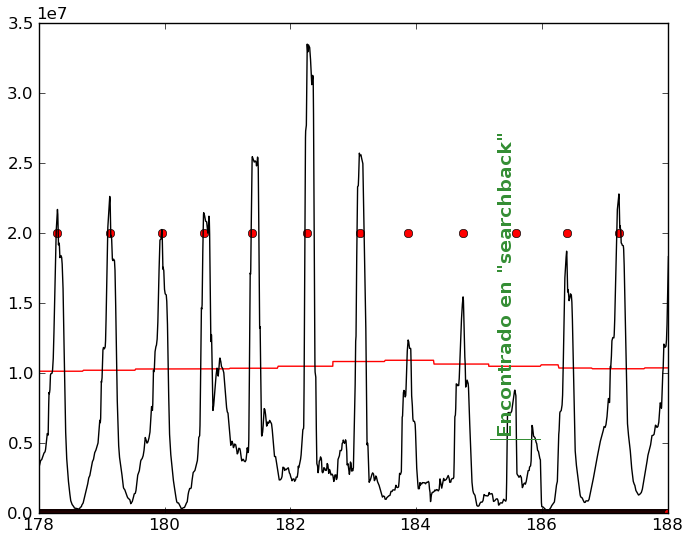
\includegraphics[width=8.5 cm]{umbral}
	\caption{Evolución de la señal}
	\label{fig:umbral}
\end{figure}

\subsubsection{Modo searchback}\label{sec:searchback}

La técnica de Search-Back consiste en la búsqueda hacia atrás de un pico R, cuando
no ha sido detectado durante un lapso de tiempo luego del pico R anterior.

Para implementar esta técnica se mantienen dos promedios del intervalo R-R. El primero
(RRAV1 ) es el promedio de los ultimos 8 intervalos R-R, es decir

\begin{equation}
RRAV_1=\frac{RR_n+...+RR_{n-7}}{8}
\end{equation}

El segundo ($RRAV_2$) es el promedio de los ultimos 8 intervalos R-R ``normales". Se le llama
normales a los intervalos RR que caen dentro de los siguientes límites:

$$RR_{low}=0.92RRAV_1$$
$$RR_{high}=1.16RRAV_1$$

Entonces el Search-Back se aplica cuando no se detecta un pico R durante un lapso de
tiempo dado por:

\begin{equation}
RR_{max}=1.16*RRAV_2
\end{equation}

Una vez en estado SearchBack, se retrocede hasta el ultimo pico encontrado. A partir de ese punto se comienza a buscar picos
R disminuyendo el umbral a la mitad (usando TH2), y actualizando los um
brales usando un peso de wpk = 0.25. Si se recuerda que el peso del umbral normal era
0.125, el efecto de este cambio es darle más importancia a los picos nuevos
El algoritmo se detiene cuando encuentra un pico R o cuando llega al punto donde entro
en Search-Back en cuyo caso decide que no hubo ningún latido. Al finalizar el algoritmo,
cualquiera sea el resultado, el umbral y la ponderación de picos nuevos vuelven a sus valores
normales.


El período refractario tiene como objeto dejar en suspenso la detección durante un
período de tiempo inmediatamente posterior a un complejo QRS donde no se espera que
aparezca otro latido dada la frecuencia cardíaca que se viene registrando. Para ello el salto
se calcula a partir del promedio de los ultimos 8 intervalos RR:

\begin{equation}
salto=\frac{RRAV_1}{4}
\end{equation}

\section{resultados}

esta implementación es capaz de funcionar ``on-line" gracias a que ninguno de los
algoritmos implicados necesita utilizar información en el fúturo con respecto a la ultima
muestra adquirida. El retardo entre la adquisición de la muestra correspondiente a un pico
R y la detección y extracción del complejo QRS es inferior a medio segundo (del orden de
algunas centenas de milisegundo).\\





% try out a theorem...
%\newtheorem{theorem}{Theorem}

%\begin{theorem}[Theorem name]
%  Consider the system ...
%\end{theorem}

%\begin{proof}
%  The proof is trivial.
%\end{proof}

% do the biliography:
%\bibliographystyle{IEEEbib}
%\bibliography{my-bibliography-file}

% where ``my-bibliography-file.bib'' is the name of the file with all the 
% BibTeX entries.

% do the biographies...
%\begin{biography}{Gregory L. Plett}
%  A bio with no face...
%\end{biography}

% If you want a picture with your biography, then specify the name of
% the postscript file in square brackets. That is, uncomment the
% following three lines and change the name of "face.ps" to the name of 
% your file.
%\begin{biography}[face.ps]{Gregory L. Plett}
%  A bio with a face...
%\end{biography}

%----------------------------------------------------------------------
% FIGURES
%----------------------------------------------------------------------
% There are many ways to include figures in the text. We will assume
% that the figure is some sort of EPS file.
%
% The outdated packages epsfig and psfig allow you to insert figures
% like: \psfig{filename.eps} These should really be done now using the
% \includegraphics{filename.eps} command.  
%
% i.e.,
%
% \includegraphics{file.eps}
%
% whenever you want to include the EPS file 'file.eps'. There are many
% options for the includegraphics command, and are outlined in the
% on-line documentation for the "graphics bundle". Using the options,
% you can specify the height, total height (height+depth), width, scale,
% angle, origin, bounding box "bb",view port, and can trim from around
% the sides of the figure. You can also force LaTeX to clip the EPS file
% to the bounding box in the file. I find that I often use the scale,
% trim and clip commands.
% 
% \includegraphics[scale=0.6,trim=0 0 0 0,clip=]{file.eps}
% 
% which magnifies the graphics by 0.6 (If I create a graphics for an
% overhead projector transparency, I find that a magnification of 0.6
% makes it look much better in a paper), trims 0 points off
% of the left, bottom, right and top, and clips the graphics. If the
% trim numbers are negative, space is added around the figure. This can
% be useful to help center the graphics, if the EPS file bounding box is
% not quite right.
% 
% To center the graphics,
% 
% \begin{center}
% \includegraphics...
% \end{center}
% 
% I have not yet written good documentation for this, but another 
% package which helps in figure management is the package ieeefig.sty,
% available at: http://www-isl.stanford.edu/people/glp/ieee.shtml
% Specify:
% 
%\usepackage{ieeefig} 
% 
% in the preamble, and whenever you want a figure,
% 
%\figdef{filename}
% 
% where, filename.tex is a LaTeX file which defines what the figure is.
% It may be as simple as
% 
% \inserteps{filename.eps}
%
% or
% \inserteps[includegraphics options]{filename.eps}
% 
% or may be a very complicated LaTeX file. 

\end{document}
